\documentclass[runningheads,a4paper]{llncs}

\usepackage{amssymb}
\setcounter{tocdepth}{3}
\usepackage{graphicx}
\usepackage{url}
\usepackage{listings}
\usepackage[linesnumbered,ruled,vlined]{algorithm2e} 

\newenvironment{itemize2}
       {\begin{itemize}
                \vspace{-0.25em}
                 \setlength{\abovedisplayskip}{0pt}
                 \setlength{\belowdisplayskip}{0pt}
                 \setlength{\itemsep}{4pt}
                 \setlength{\parskip}{0pt}
                 \setlength{\parsep}{0pt}
                 \setlength{\topsep}{0pt}
                 \setlength{\partopsep}{0pt}
         }
         {\vspace{-0.25em}
         \end{itemize}}
}

\newenvironment{enumerate2}
       {\begin{enumerate}
                \vspace{-0.25em}
                 \setlength{\abovedisplayskip}{0pt}
                 \setlength{\belowdisplayskip}{0pt}
                 \setlength{\itemsep}{4pt}
                 \setlength{\parskip}{0pt}
                 \setlength{\parsep}{0pt}
                 \setlength{\topsep}{0pt}
                 \setlength{\partopsep}{0pt}
         }
         {\vspace{-0.25em}
         \end{enumerate}}
}

\urldef{\mailsa}\path|{Firstname.Lastname}@springer.com|    
\newcommand{\keywords}[1]{\par\addvspace\baselineskip
\noindent\keywordname\enspace\ignorespaces#1}

\begin{document}

\mainmatter  

\title{Serelex: Search and Visualization of Semantically Related Words}

\titlerunning{Serelex: Search and Visualization of Semantically Related Words}

\author{Alexander Panchenko\inst{1,2} \and Pavel Romanov\inst{2} \and Olga Morozova\inst{1} \and Hubert Naets\inst{1} \and Andrey Philippovich\inst{2} \and Alexey Romanov\inst{2} \and C\'{e}drick Fairon\inst{1}}


\authorrunning{Alexander Panchenko et al.}

\institute{  Universit\'{e} catholique de Louvain, Louvain-la-Neuve, Belgium 
\url{{Firstname.Lastname}@uclouvain.be}   
\and
Bauman Moscow State Technical University, Moscow, Russia
%\mailsa\\
%\mailsb\\
%\mailsc\\
\url{{promanov,aphilippovich,aromanov}@it-claim.ru}
}

\toctitle{ \ldots } 
\tocauthor{ \ldots }
\maketitle

\begin{abstract}

We present Serelex, a system that provides, given a query in English, a list of semantically related words. The terms are ranked according to an original semantic similarity measure learnt from a huge corpus. The system performs comparably to dictionary-based baselines, but does not require any semantic resource such as WordNet. Our study shows that users are completely satisfied with  70\% of the query results.     


\keywords{ semantic similarity measure, visualization, extraction.}
\end{abstract}


\section{Introduction}

We present \textit{Serelex}, a system that, given a query in English, returns a list of related terms ranked according to a \textit{semantic similarity measure}. The system helps to learn the meaning of a query term and to discover semantically similar words in an interactive way. Unlike dictionaries and thesauri (e.g., \url{Thesaurus.com} or \url{VisualSynonyms.com}), \textit{Serelex} relies on information extracted from text corpora. In comparison to other similar systems (e.g., BabelNet~\footnote{ \url{http://lcl.uniroma1.it/bnxplorer/}}, ConceptNet~\footnote{ \url{http://conceptnet5.media.mit.edu/}}, UBY~\footnote{\url{https://uby.ukp.informatik.tu-darmstadt.de/webui/tryuby/}}), \textit{Serelex} does not depend on a semantic resource like WordNet. Instead, we build upon an original pattern-based similarity measure~\cite{panchenko2012konvens}. The proposed system
has a precision rate comparable to those of the 9 baselines. Furthermore, it has a larger lexical coverage than the dictionary-based systems, provides list-, graph-, and image-based GUIs, and is open source. 

%Finally, it is automatically updated with relations extracted from new documents.    

%\url{http://www.lexfn.com/}
%UWN (Universal WordNet): \url{http://www.lexvo.org/uwn/}

%In general: 
%\url{http://www.tesaurus.ru}
%\url{http://www.eat.rl.ac.uk/}

%Visual:
%\url{JeuxDeMots.org}, 
%Slovesa~\footnote{\scriptsize \url{http://www.slovesa.ru/}}
%Данный вид интерфейса в был реализован в некоторых проектах и показал свою эффективность при визуализации лексико-семантических сетей:
%\url{http://visualworld.ru/search.jsp}
%\url{http://about.viwo.ru/semantic.html}
%\url{http://visualworld.ru/search.jsp}.  
%\url{http://dev.sigwp.org/WikiVisSL.Web/Visualizer.aspx}
%\url{http://www.touchgraph.com/seo} 

%Such systems measure semantic similarity of terms. 

\section{The System}

Serelex is freely available online~\footnote{ \url{http://serelex.cental.be}, available under conditions of LGPLv3 license.}. Figure~\ref{fig:architecture} presents its structure, which consists of an extractor, a server and a user interface. The extractor gathers semantic relations between words from a raw text corpus. The extraction process occurs offline. The extracted relations are stored in the database. The server provides fast access to the extracted relations over HTTP. A user interacts with the system through a web interface or an API. %The system as well as the data and the evaluation scripts are open source.

%~\footnote{ \url{http://serelex.cental.be/page/about}, available under conditions of LGPLv3.}.

\begin{figure}
	\centering
		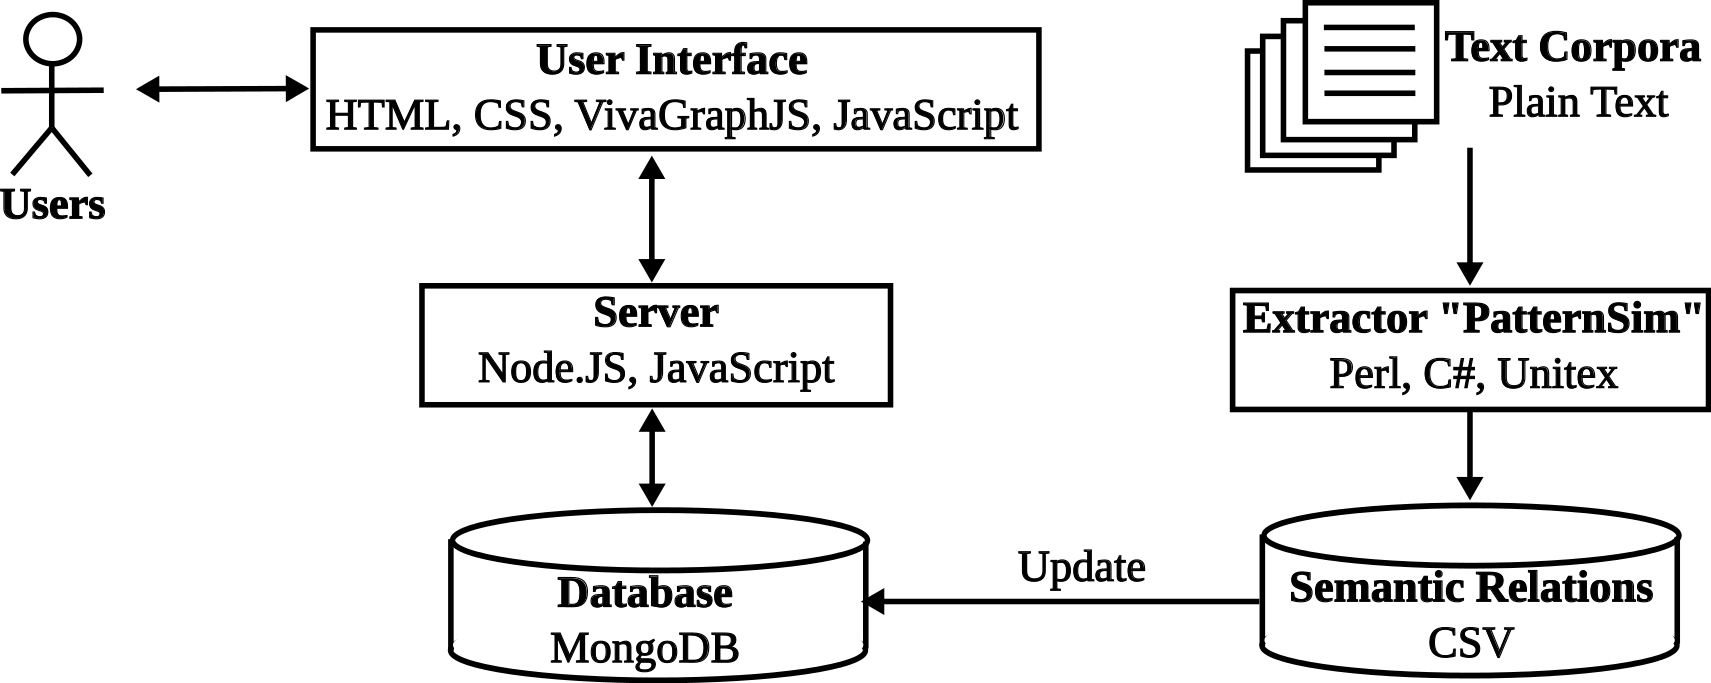
\includegraphics[width=0.60\textwidth]{figures/arch2} 
		\caption{Structure of the system \textit{Serelex}.}
			\label{fig:architecture}
\end{figure}


\textbf{Extractor.} The extractor is based on the semantic similarity measure \textit{PatternSim} and \textit{Efreq-Rnum-Cfreq-Pnum} re-ranking formula~\cite{panchenko2012konvens}. 
This corpus-based measure relies on handcrafted lexico-syntactic patterns which extract concordances. Similarity score is proportional to the number of term co-occurrences within those concordances, e.g.: \texttt{ \footnotesize such \{non-alcoholic [sodas]\} as \{[root beer]\} and \{[cream soda]\}}. The score is normalized with term frequencies and other extraction statistics~\cite{panchenko2012konvens}. We used as a  corpus a combination of Wikipedia abstracts and ukWaC~\cite{baroni2009wacky}  (5,387,431 documents, 2.915 $\cdot 10^9$ tokens, 7,585,989 lemmas, 17.64 Gb). 
%Processing of the corpus took around 70 hours on a standard machine (Intel i5, 4Gb RAM, HDD 5400rpm). which takes into account frequencies of extraction, number of extracted relations of a term, frequency of a term in the corpus, and number of distinct patterns extracted a relation.
The result of the extraction is 11,251,240 untyped semantic relations (e.g., $\langle Canon, Nikon, 0.62 \rangle$) between 419,751 terms. 
 
\textbf{Server.} The server returns a list of related words for each query, ranked according to their semantic similarity measure stored in the database. The queries are lemmatized with the DELA dictionary~\footnote{\url{http://infolingu.univ-mlv.fr/}, available under conditions of LGPLLR.}. An approximate search is performed for queries with no results. The system can import networks in CSV format created by other similarity metrics and extractors. 

\textbf{User Interface.} One can access the system via a graphical user interface or a RESTful API. The GUI  consists of three key elements: a search field, a list of the results and a graph of the results (see Fig.~\ref{fig:gui}). A user  interacts with the system by issuing a query -- a single word such as ``mathematics'' or a multiword expression such as ``computational linguistics''. Query suggestions are sorted at the same time by term frequency in the corpus, by query frequency, and alphabetically. A list of results contains 20 terms which are the most semantically related to the query. The graph of results provides an alternative representation of the toplist. It enables visualization of semantic relations with a force-directed graph layout algorithm based on the Barnes-Hut simulation~\cite{barnes1986hierarchical}. The layout incorporates the secondary relations: words related to the words linked to the query. This lets the layout algorithm cluster the results. A user can issue additional queries by clicking on the nodes. the system can also visualize the results as a set of images. 

\begin{figure}
	\centering
		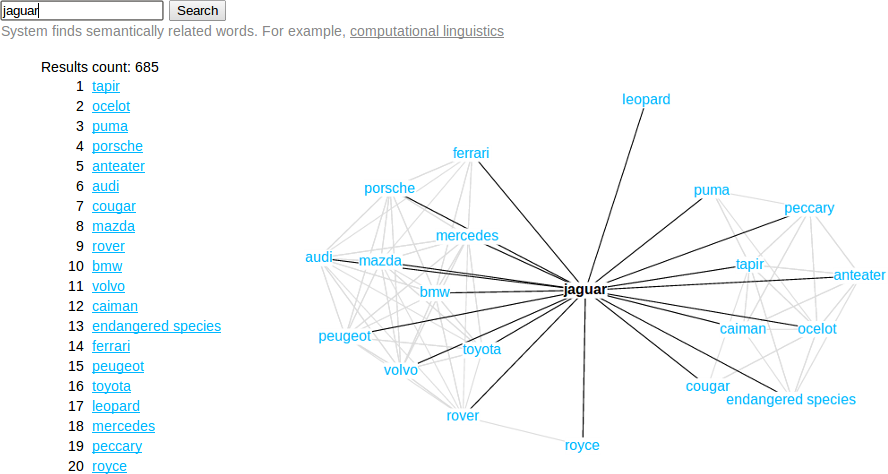
\includegraphics[width=0.80\textwidth]{figures/jaguar} 
		\caption{Graphical user interface of the \textit{Serelex} system: results of the query ``jaguar''.}
			\label{fig:gui}
\end{figure}

\section{Evaluation and Results}

We evaluated the system against four tasks (see~\cite{panchenko2012konvens} for details): 
%Three established approaches to semantic similarity are based on WordNet, dictionaries and corpora. WordNet-based measures such as \textit{WuPalmer}~\cite{wu1994verbs}, \textit{LeacockChodorow}~\cite{leacock1998} and \textit{Resnik}~\cite{resnik1995} achieve a high precision, but suffer from a limited coverage. Dictionary-based methods such as \textit{ExtendedLesk}~\cite{banerjee2003extended}, \textit{GlossVectors}~\cite{patwardhan2006using} and \textit{WiktionaryOverlap}~\cite{zesch2008extracting} have similar properties as they rely on manually-crafted resources. Corpus-based measures such as \textit{ContextWindow}~\cite{cruys2010mining}, \textit{SyntacticContext}~\cite{cruys2010mining} or~\textit{LSA}~\cite{landauer1998introduction} provide a decent coverage as they derive similarity scores directly from a corpus. However, these measures suffer from a lower precision as they rely on a simple representation based on the vector space model.

%To overcome shortcomings of the existing systems, we build upon an  original pattern-based similarity measure~\cite{panchenko2012konvens}. The proposed system performs comparably to the baselines, but requires no semantic resources such as WordNet. Furthermore, it has better lexical coverage than the dictionary-based systems, provides an original graph-based GUI, and is open source. 

1. \textbf{Correlation with Human Judgements.} We used standard datasets (MC, RG, WordSim) to  measure Spearman's correlation with human judgements. Our system performs comparably to the baselines, that includes 3 WordNet-based measures (\textit{WuPalmer}~\cite{wu1994verbs}, \textit{LeacockChodorow}~\cite{leacock1998}, \textit{Resnik}~\cite{resnik1995}), 3 dictionary-based measures (\textit{ExtendedLesk}~\cite{banerjee2003extended}, \textit{GlossVectors}~\cite{patwardhan2006using}, \textit{WiktionaryOverlap}~\cite{zesch2008extracting}), and 3 corpus-based measures (\textit{ContextWindow}~\cite{cruys2010mining}, \textit{SyntacticContext}~\cite{cruys2010mining}, ~\textit{LSA}~\cite{cruys2010mining}).

2. \textbf{Semantic Relation Ranking.} This task relies on a set of semantic relations (BLESS,  SN) to estimate \textit{relative} precision and recall of each measure. The precision of \textit{Serelex}  is comparable to the 9 baselines, but its recall is seriously lower due to the sparsity of the pattern-based approach (see Figure~\ref{fig:eval} (a)). 

3. \textbf{Semantic Relation Extraction.} We estimated the precision of the extracted relations for 49 words (the vocabulary of the RG dataset). Three annotators indicated whether the terms are semantically related or not. Each of them was asked to label each result from the top 50 as relevant or irrelevant. We calculated extraction precision at $k = \{1, 5, 10, 20, 50\}$. Average precision varies between 0.736 for the top relation and 0.599 for the top 50 (see Figure \ref{fig:eval} (b)). The inter-raters agreement in terms of Fleiss's kappa is substantial (0.61-0.80).

4. \textbf{User Satisfaction.} We also measured user satisfaction with our results. 23 assessors were asked to issue 20 queries of their choice and, for each of them, to rank the top 20 results as relevant, irrelevant, or a mix of both. We collected 460 judgements from the 23 assessors and 233 judgements from 109 anonymous users (see Fig.~\ref{fig:eval} (c)). Users and assessors (users asked to assess the system) issued together 594 distinct queries. According to this experiment, the results are relevant in 70\% of the cases and irrelevant in 10\% of the cases. %Finally, 20\% of queries recall both relevant and irrelevant results. 

\section{Conclusion}

We presented a system which finds semantically related words. Our results have shown that it has a precision comparable to the dictionary-based baselines and a better coverage as it extracts relations directly from texts. The system achieves a Precision@1 of around 74\%, and users are satisfied with 70\% of the query results without the need for any manually-crafted dictionary.

\begin{figure}
	\centering
		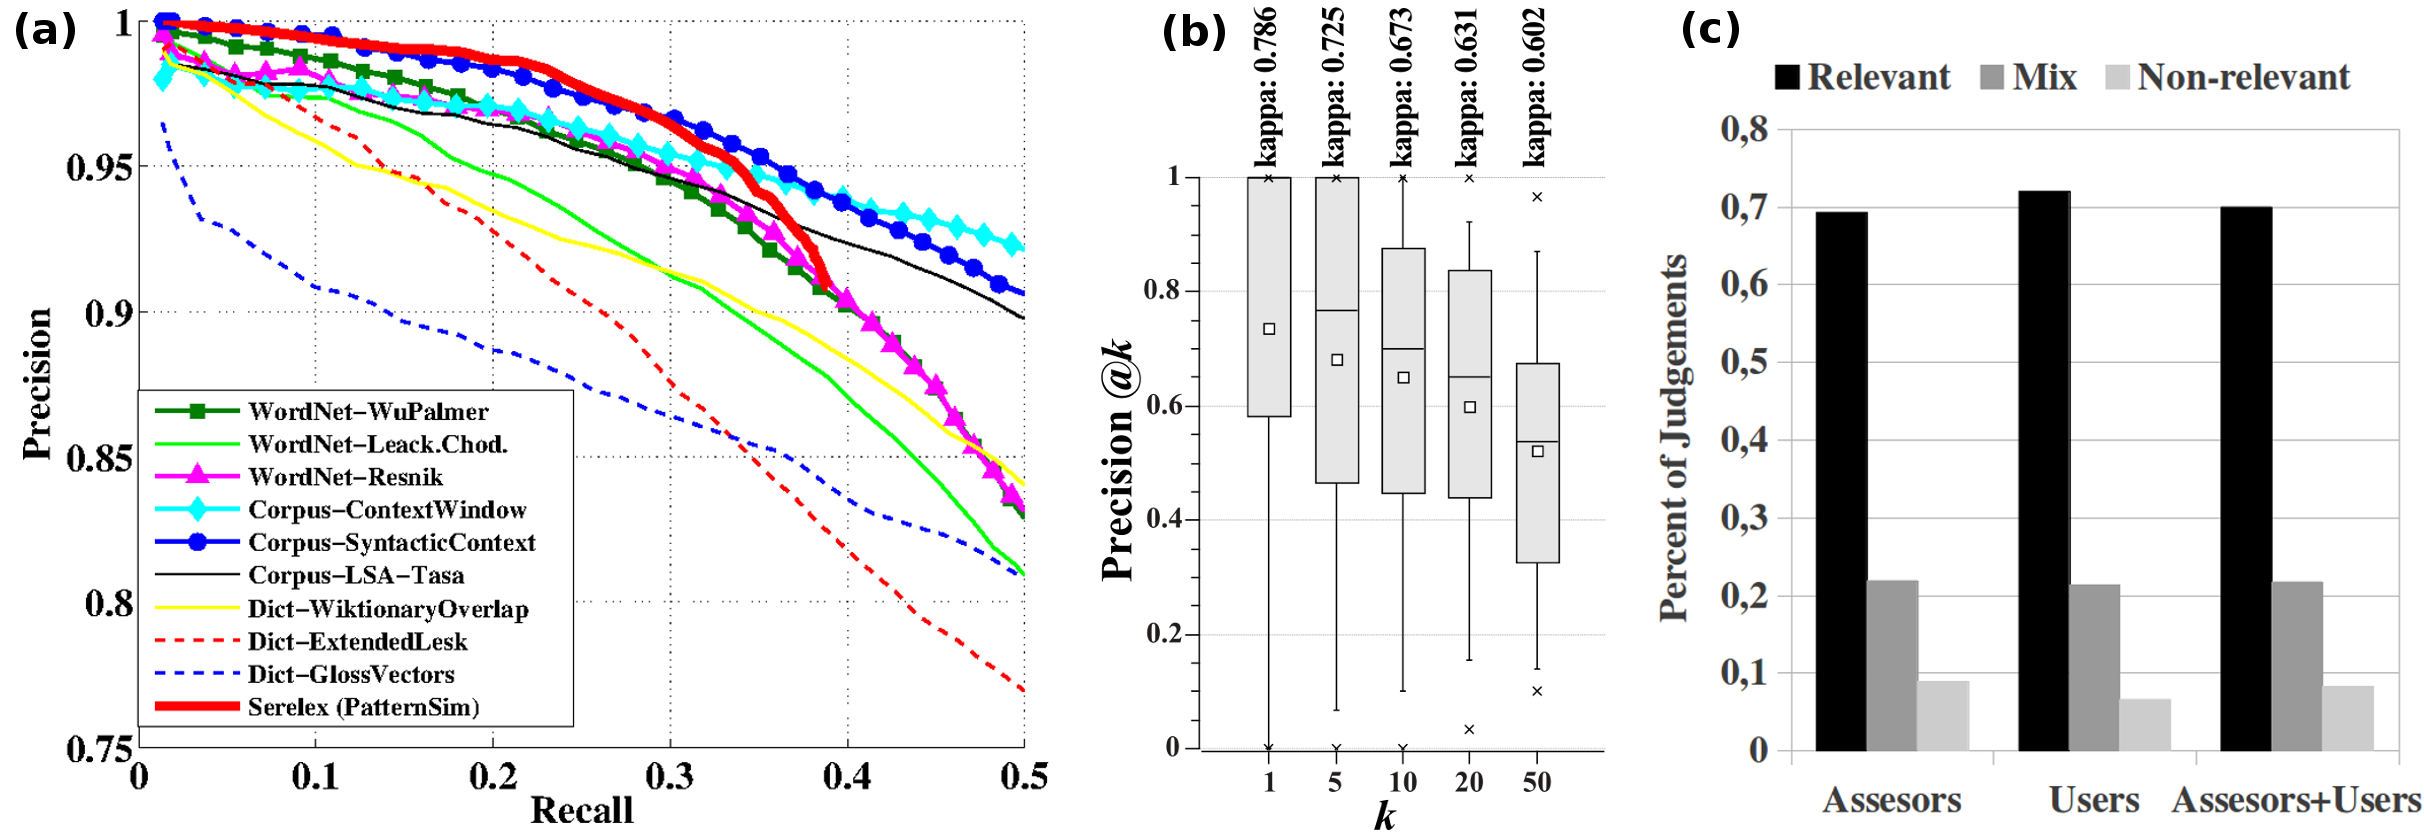
\includegraphics[width=1.0\textwidth]{figures/eval2}		
		\caption{ Evaluation: (a) precision-recall graph of the semantic relation ranking task on BLESS; (b) semantic relation extraction task; (c) users' satisfaction of top 20 results. }
	\label{fig:eval}
\end{figure}

\bibliographystyle{splncs}
\bibliography{biblio2}

\end{document}
